\documentclass[a4paper]{ctexart}
\usepackage{amsmath, amsthm, amssymb, graphicx}
\usepackage{setspace}
%\usepackage[bookmarks=true, colorlinks, citecolor=blue, linkcolor=black]{hyperref}

% 导言区

\title{C++程序设计大作业报告}
\date{\today}
\pagestyle{plain}
\begin{document}
        \thispagestyle{empty}
    	\begin{figure}[t]
		\parbox[b]{2cm}{
			}
		\parbox[b]{9cm}{
			\begin{center}

				%\small \textbf{SOUTHEAST\quad UNIVERSITY} 
			\end{center}
			}
	\end{figure}

	\begin{center}
		\quad \\
		\quad \\
		\heiti \fontsize{25}{17} 程\quad 序\quad 设\quad 计\quad 大\quad 作\quad 业\quad 报\quad 告
		\vskip 2.5cm
		\heiti \zihao{2} 	
	\end{center}
	\vskip 2.5cm

	\begin{quotation}
		\songti \fontsize{15}{15}
		\doublespacing
		\par\setlength\parindent{12em}
		\quad 

        作业名称:\underline{\quad 城市天际线\quad}


		学\hspace{0.61cm} 院:\underline{\quad 材料学院\qquad}
        
        班\hspace{0.61cm} 级:\underline{\qquad 04102301\quad}

		学生姓名:\underline{\qquad 白昊明\qquad }

		学\hspace{0.61cm} 号:\underline{\quad 2023301350\quad}

		\vskip 2cm
        \centering
		西北工业大学
		\vskip 0cm
		\centering
		2023年12月2日
	\end{quotation}
    \textbf{}
    \begin{abstract}
        本次大作业选择的是上的ACM模拟试题,题目的主要要求是根据给出的矩形建筑物的上沿,输出城市的天际线的顶点向量。
		本次作业使用了C++风格的文件流操作,代码更加简洁易懂,并且融入了面向对象编程的思想。
		本次作业基本完成既定目标,实现了预期功能,但是对数据执行了三次循环,执行效率尚有待提高。
		本次作业思路清晰明确,运用了高级工具,运用了C++特有的功能和特性。
    \end{abstract}
    \newpage

	\tableofcontents
	\newpage
	\section{摘要}
	\subsection{设计题目}
	英文名称:Skyline

	中文名称:城市天际线
	\subsection{设计内容}
	本项目来自 onlinejudge.org (即 Valladolid Programming Contest Site 的OJ题库)
	\paragraph{英文原文}~

	Draw the skyline of a city according to the data given by the input file.
	
	With the advent of high speed graphics workstations, CAD (computer-aided design) and other areas (CAM, VLSI design) have made increasingly effective use of computers. One of the problems with drawing images is the elimination of hidden lines — lines obscured by other parts of a drawing.

	You are to design a program to assist an architect in drawing the skyline of a city given the locations of the buildings in the city. To make the problem tractable, all buildings are rectangular in shape and they share a common bottom (the city they are built in is very flat). The city is also viewed as two-dimensional. A building is specified by an ordered triple ($L_i$, $H_i$, $R_i$) where $L_i$ and $R_i$ are the left and right coordinates, respectively, of building $i$ (0 $\textless$  $L_i$ $\textless$  $R_i$) and $H_i$ is the height of the building. In the diagram below buildings are shown on the left with triples.

	(1,11,5),(2,6,7),(3,13,9),(12,7,16),(14,3,25),(19,18,22),(23,13,29),(24,4,28)

	The skyline, shown on the right, is represented by the sequence:

	(1,11,3,13,9,0,12,7,16,3,19,18,22,3,23,13,29,0)

	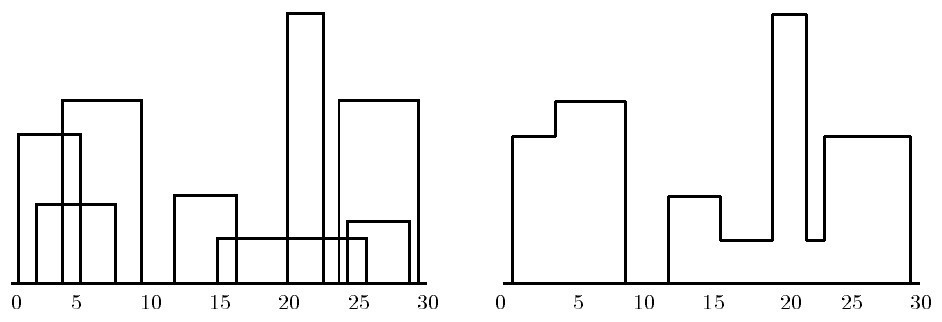
\includegraphics[width=10.465cm,height=3.577cm]{effect.jpg}

	\textbf{Input}

	The input is a sequence of building triples. All coordinates of buildings are integers less than 10,000 and there will be at least one and at most 5,000 buildings in the input file. Each building triple is on a line by itself in the input file. All integers in a triple are separated by one or more spaces. The triples will be sorted by Li, the left x-coordinate of the building, so the building with the smallest left x-coordinate is first in the input file.

	\textbf{Output}

	The output should consist of the vector that describes the skyline as shown in the example above.
	
	In the skyline vector ($v_1$,$v_2$,$v_3$,...,$v_n-2$,$v_n-1$,$v_n$), the $v_i$ such that $i$ is an even number represent a horizontal line (height). The $v_i$ such that $i$ is an odd number represent a vertical line (x-coordinate). The skyline vector should represent the "path" taken, for example, by a bug starting at the minimum x-coordinate and traveling horizontally and vertically over all the lines that define the skyline. Thus the last entry in all skyline vectors will be a '0'.
	
	\textbf{Sample Input}

	1 11 5

	2 6 7

	3 13 9

	12 7 16

	14 3 25

	19 18 22

	23 13 29

	24 4 28

	\textbf{Sample Output}

	1 11 3 13 9 0 12 7 16 3 19 18 22 3 23 13 29 0



	\paragraph{中文翻译}~

	根据输入文件中给出的数据描绘一个城市的天际线。

	随着高速计算机的流行,CAD(计算机辅助设计软件)和其他的领域(CAM,VLSI设计等)已经越发高效地使用着计算机。图形绘制中,怎样消去隐藏的直线——即那些被绘制图形的其他部分遮挡的直线——是一个问题。

	你将要设计一个程序以辅助建筑师通过输入城市中建筑的位置描绘城市的天际线。为了简化这个问题,我们假设所有的建筑都是矩形并且它们的底部高度相同(这个城市的地面非常的平坦)。同样地,城市也被看作一个二维的平面(正垂面)。在题目中,每座建筑都用一组三元数据表示 ($L_i$, $H_i$, $R_i$) 。其中,$L_i$和$R_i$分别表示建筑 $i$ 两侧边的所在位置的横坐标。下方示意图中的建筑可以用如下的一行三元数据表示:

	(1,11,5),(2,6,7),(3,13,9),(12,7,16),(14,3,25),(19,18,22),(23,13,29),(24,4,28)

	而图中右半部分展示的天际线则可以用如下的一组数列表示:

	(1,11,3,13,9,0,12,7,16,3,19,18,22,3,23,13,29,0)
	
	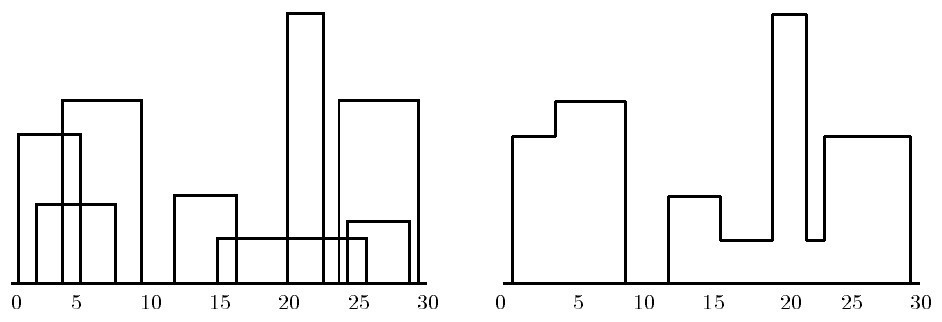
\includegraphics[width=10.465cm,height=3.577cm]{effect.jpg}

	\textbf{输入}
	
	输入的是是一个表示建筑的三元数据的序列。所有的坐标值都是小于10000的整数并且输入文件中建筑的数量不会超过5000座。每一座建筑的坐标数据和它在输入文件中独立成行。同一组数据的两个整数之间用一个或者几个空格分隔。数据已经根据$L_i$从小到大排序,所以有着最小的横坐标的建筑将会第一个出现在输入文件中。

	\textbf{输出}

	输出应该包含如案例中的用来描绘城市天际线的向量。

	在天际线向量中 ($v_1$,$v_2$,$v_3$,...,$v_n-2$,$v_n-1$,$v_n$),当$i$是一个偶数时,$v_i$表示天际线的高度而当$i$是奇数时,$v_i$表示天际线中竖线的横坐标。天际线向量实际上表示的是天际线的“路径”。假设一个爬虫根据这些向量的终点水平或者竖直的爬行,那么这个爬虫经过的轨迹就是所需的天际线。因此,向量的最后一个坐标的值为‘0’。

	\textbf{输入样例}

	1 11 5

	2 6 7

	3 13 9

	12 7 16

	14 3 25

	19 18 22

	23 13 29

	24 4 28

	\textbf{输出样例}

	1 11 3 13 9 0 12 7 16 3 19 18 22 3 23 13 29 0


	\subsection{开发工具}
	本项目的开发环境如下:

	OS: Ubuntu 22.04.3 LTS on Windows 10 x86\_64

	Kernel: 5.15.133.1-microsoft-standard-WSL2

	CC: gcc (Ubuntu 11.4.0-1ubuntu1$\sim$22.04) 11.4.0

	Text Editor: VIM - Vi IMproved 8.2

	Debuger: GNU gdb (Ubuntu 12.1-0ubuntu1$\sim$22.04) 12.1
	\subsection{应用平台}
	本项目基于Linux x86\_64 ,但是经测试,在 Windows 11 x86\_64 上使用编译通过并且可以正常运行。本项目未在 WindowsXP 等操作系统上进行测试,但是考虑到最新版本的 Code::Blocks 自带 GCC 8.1 编译器并且提供了对于 WindowsXP 的支持,而项目中使用的以变量作为数组长度初始化数组等行为最早出现在 C++ 11 标准并且 GCC 从 GCC 4.8.1 开始支持 C++ 11 ,我们可以推测,本项目可以在 WindowsXP 上编译并运行。但是,我们不能确定本项目是否可以支持 Windows 2000 ,Windows 98 等较早的 Windows 版本。
	\section{详细设计}
	本程序的基本流程如下:

	1、通过C++的文件流相关函数,获取输入文件。

	2、计算输入文件的行数(考虑到在理想无误的输入文件中,每一行都只有一组输入数据,我们可以根据行数计算输入数据的长度)。

	3、建立一个数组,将输入文件中的数据存放在数组当中。

	4、逐个分析数组中的数据,并且根据这些数据得到各个坐标处,城市天际线的高度。

	5、分析天际线,得到并输出所需要的关键向量。
	\subsection{程序结构}
	本项目源代码共有三个文件,分别为 file.h, algorithm.h 和 main.cpp ,但是我们可以将三个文件的代码合并到一个文件当中,并不会冲突影响。分居多个文件的目的是为了使代码结构更加清晰,避免过度复杂,同时也方便将程序模块化,也为之后在实际的应用中方便移植改造。
	\subsection{主要功能}
	本项目的主要功能如下:
	
	从一个输入文件读取城市建筑的信息,获取其位置和高度。获得城市的天际线数据,并且将数据简化,得到所需要的向量序列,并且在屏幕上输出。本程序具有模块化,可移植等特性,每个函数都可以被单独引用,相互之间依赖少,结构简单,清晰。
	\subsection{函数实现}
	\paragraph{int countline}
	以文件名或文件路径(C语言风格字符串)作为参数。新建一个输入文件流,命名为ReadFile,一个整数表示文件的行数,根据文件路径打开文件。首先使用.fail函数测试文件路径的有效性,若无效,则返回-1。然后,根据文件流每被读取一次,指针就会向后方移动的特点,使用getline函数操作ReadFile,当getline函数返回非0(非 EOF )时,我们就让n自增一次,代表读取一行。当读取到EOF之后,关闭文件防止内存泄漏,返回n。
	\paragraph{int readfile}
	本函数的参数有:C++风格的字符串filename表示文件名,整数型数组d[][3]用于存储数据,整数linenum表示文件行数。在这个函数中,通过数组作为函数形式参数时传递指针常量而非数组数据的特点,实现了返回多值的功能。首先,因为数组的操作不够便利,同时可移植性也不够强,在编写程序时,我先新建三个int ** 指针,名称分别为p,n,x。然后我使用malloc命令给n指针分配内存并将p,x赋值为n以保护n不在后续操作中丢失,造成内存泄露。然后,我通过p将d[n]赋值给*(n+i)。再使用readfile表示文件输入流,整数变量m表示城市的长度(横坐标最大值),利用fin.getline函数,将每行文件:1、输入字符串buff 2、用sscanf输入数据到*(x),*(x+1),*(x+2),然后令x自增,获取所有数据。在获取数据时,将右侧坐标与m比较,若坐标值大于m,则将m的值变为新的右侧坐标的值。最后,返回m作为城市的长度,也就是天际线的最后一个横坐标 ($v_{n-1}$) 。
	\paragraph{void dataprocess}
	本函数需要两个输入参数:int *bitmap 和 int *rectan ,其中,bitmap指针后方有长度大小(单位为整数的存储空间大小)为整个城市长度大小(最大坐标大小)的内存,用于存储在某座标处的最大高度*rectan指针则代表了一个长度为3的数组,存放给出的三元数据,可以表示出建筑的矩形轮廓。这个函数的功能是描绘每个矩形的天际线,并且消去已经过时的天际线。函数在实现时,将bitmap移到*rectan的位置,然后逐个比较*bitmap和*(rectan+1)的大小,若测得*(rectan+1)更大,则*(bitmap)赋值为*(rectan+1),并且对*(bitmap)自增,重复直到bitmap等于输入时的bitmap+*(rectan+2)。注:指针加上一个整数表示其后方的第n个存储空间。
	\paragraph{void key\_vector}
	这个函数的输入值有:int* p 和 int length ,这两个参数分别表示城市的天际线和城市的长度。函数的实现原理为:将p$[$i$]$和p$[$i+1$]$比较,若更改,则输出一个关键向量,最后换行。
	\paragraph{int main}
	主函数是整个程序的主体,负责整合,调用几个函数,并且实现相应的功能。输入文件文件名默认为inputfile,但是也可以通过简单的修改,实现输入文件路径的功能。

	首先,主函数初始化整数linenum,并调用readfile给linenum赋值。
	
	当文件读取正常时,初始化length整数,data$[$linenum$][3]$,调用readfile函数给length赋值,并将数据存入data数组。
	
	然后我们新建bitmap数组,调用data\_process函数将bitmap绘制完成。

	最后,调用key\_vector函数,输出结果,并返回0表示正常退出。
	\paragraph{read\_data}
	这个函数的功能是逐行输出得到的数据,并未使用,仅用于调试。
	\subsection{开发日志}
	本项目从
	\section{程序调试及运行}
	\subsection{程序运行结果}
	\subsection{程序使用说明}
	\subsection{程序开发总结}
	\section{附件(源程序)}

\end{document}